\mychapter{Procedimentos Metódicos}
\label{Cap:ProcedimentosMetodicos}

O Capítulo \ref{Cap:ProcedimentosMetodicos} descreve os procedimentos metodológicos adotados no desenvolvimento da plataforma DDR, detalhando as etapas do processo de implementação, as ferramentas e tecnologias utilizadas, e os métodos aplicados para garantir a qualidade e eficiência do sistema.

\section{Desenvolvimento do Sistema DDR}

O desenvolvimento da plataforma DDR foi realizado seguindo uma abordagem iterativa e incremental, baseada no método ágil \textit{Scrum}. Essa abordagem permitiu uma adaptação constante às necessidades do projeto, com entregas frequentes e revisões contínuas, assegurando que o sistema atendesse aos requisitos funcionais e não funcionais previamente estabelecidos.

\subsection{Arquitetura do Sistema}

A arquitetura do DDR foi projetada para garantir escalabilidade, modularidade e alto desempenho. O sistema foi desenvolvido utilizando uma arquitetura cliente-servidor, com o \textit{front-end} e o \textit{back-end} sendo implementados separadamente, garantindo uma maior flexibilidade e manutenibilidade.

O \textit{front-end} foi implementado utilizando a biblioteca \textbf{React.js}, que oferece uma interface de usuário dinâmica e responsiva, capaz de lidar com a visualização de grandes volumes de dados em tempo real. A arquitetura \textbf{React} baseada em componentes permitiu a reutilização de código, tornando o sistema mais modular e facilitando a manutenção e escalabilidade. O desenvolvimento da solução foi aprimorada com a utilização de \textbf{TypeScript}, um \textit{superset} ao JavaScript que oferece tipagem estática, garantindo maior segurança e previsibilidade no desenvolvimento.

O \textit{back-end} foi desenvolvido utilizando \textbf{Python}, o que permitiu uma implementação eficiente, especialmente em relação ao processamento assíncrono de grandes volumes de dados industriais. O uso de \textbf{FastAPI}, uma \textit{framework} moderna para a criação de APIs RESTful, garantiu a comunicação rápida e segura entre o \textit{front-end} e o \textit{back-end}. O Python também foi utilizado para a execução dos cálculos de reconciliação de dados, aproveitando bibliotecas como \textbf{NumPy} e \textbf{SciPy} para a resolução de problemas de otimização multivariáveis.

\subsection{Modelagem e Reconciliação de Dados}

A reconciliação de dados foi implementada com base no \textbf{método dos multiplicadores de Lagrange}, que é amplamente utilizado para resolver problemas de otimização multivariáveis com restrições. Este método foi aplicado para ajustar os dados de medição provenientes dos sensores industriais, assegurando que os resultados estivessem em conformidade com as leis de conservação de massa e energia.

Durante o processo de reconciliação, os dados de entrada eram validados e ajustados de forma a minimizar os erros sistemáticos e aleatórios presentes nas medições. A aplicação deste método foi crucial para garantir a consistência dos dados e a confiabilidade dos resultados, especialmente em ambientes industriais onde medições imprecisas podem comprometer a eficiência dos processos produtivos.

\section{Ferramentas Utilizadas no Desenvolvimento}

\subsection{React.js e TypeScript no Front-End}

O \textbf{React.js} foi escolhido para o desenvolvimento da interface do DDR devido à sua eficiência no gerenciamento de interfaces dinâmicas e na manipulação de grandes volumes de dados em tempo real. Sua arquitetura baseada em componentes reutilizáveis facilitou a manutenção do sistema e garantiu escalabilidade, essenciais para o ambiente industrial. A adoção de \textbf{TypeScript} acrescentou uma camada adicional de segurança, permitindo a detecção de erros durante o desenvolvimento e aumentando a confiabilidade e robustez do código.

\begin{figure}[htbp!]
    \begin{center}
        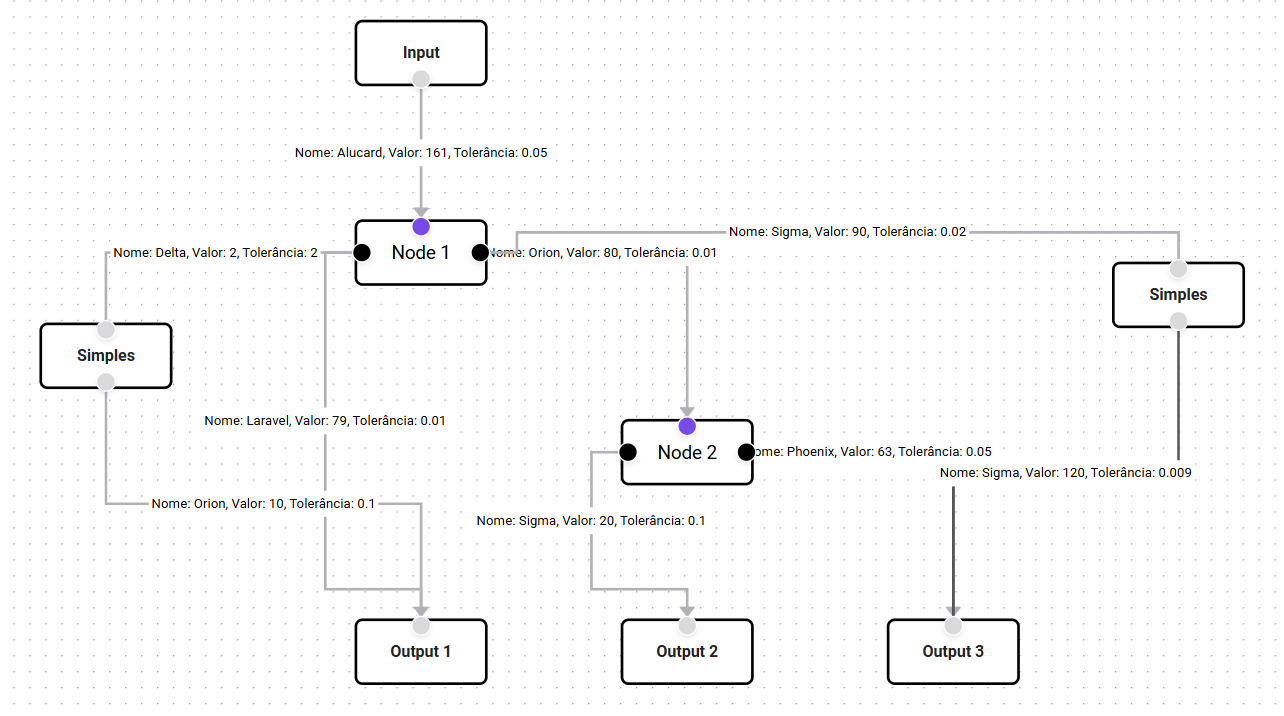
\includegraphics[width=0.75\textwidth]{figuras/reactflow.png}
        \caption{Exemplo de uma modelagem com o ReactFlow.}
        \label{fig:ReactFlowPicture}
    \end{center}
\end{figure}

Um elemento crucial no \textit{front-end} foi a utilização da biblioteca \textbf{ReactFlow}, especializada na criação de diagramas interativos. Ela proporcionou uma visualização clara dos fluxos de dados industriais, permitindo que operadores e engenheiros modelassem e monitorassem processos complexos diretamente na interface do DDR. A biblioteca foi adaptada com diversas funcionalidades personalizadas, como a extração de matrizes de incidência das conexões entre nódulos, facilitando a análise das relações entre variáveis industriais.

Essas adaptações permitiram que o ReactFlow atendesse às demandas específicas da modelagem industrial, tornando-o uma ferramenta eficiente para o controle visual de processos.

\subsection{Python no Back-End}

O \textbf{Python} foi escolhido para o \textit{back-end} do DDR devido à sua flexibilidade e eficiência no processamento de grandes volumes de dados e operações assíncronas. A combinação de \textbf{FastAPI} com \textbf{NumPy} permitiu a execução eficiente de cálculos complexos, essenciais para os processos de reconciliação de dados, enquanto o \textbf{SQLAlchemy} foi utilizado para gerenciar a comunicação com o banco de dados \textbf{PostgreSQL}, garantindo integridade e performance nas operações de leitura e escrita.

A arquitetura do \textit{back-end} foi projetada com base no \textit{framework} \textbf{Flask}, criando um servidor leve e escalável, com três rotas principais em padrão RESTful:

\begin{itemize}
    \item \textbf{/reconcile}: Responsável por processar os dados de reconciliação. O cliente pode enviar tanto dados em tempo real quanto em bateladas para que o servidor aplique os algoritmos de reconciliação e retorne os dados corrigidos, o qual se comunica com as funções de minimização de multivariáveis aplicando o método de Lagrange.
    \item \textbf{/reconciled\_data}: Realiza consultas ao banco de dados \textbf{PostgreSQL} para recuperar e fornecer ao cliente os dados já reconciliados, garantindo o acesso contínuo às informações processadas.
    \item \textbf{/health}: Verifica o \textit{status} do sistema, monitorando a saúde do servidor e sua conexão com o banco de dados, assegurando a estabilidade e disponibilidade da plataforma.
\end{itemize}

Essa arquitetura permite uma integração eficiente entre o \textit{front-end} e o \textit{back-end}, garantindo a escalabilidade e o desempenho da plataforma em ambientes industriais complexos.


\subsection{Banco de Dados PostgreSQL}

O \textbf{PostgreSQL} foi adotado no DDR devido à sua robustez, escalabilidade e adequação ao gerenciamento de grandes volumes de dados industriais. Sua capacidade de lidar com consultas complexas e realizar operações matemáticas avançadas torna-o ideal para armazenar e processar dados contínuos provenientes de sensores industriais, garantindo integridade e segurança nas operações de reconciliação.

A eficiência do \textbf{PostgreSQL} é reforçada por seus recursos avançados de indexação, como \textit{B-tree} e \textit{hash indexes}, que permitem uma rápida recuperação de dados, otimizando consultas complexas e cálculos em grandes matrizes sem comprometer o desempenho do sistema.

A estrutura de dados no banco foi projetada para garantir integridade e rastreabilidade, com a tabela principal de reconciliação contendo as seguintes colunas:

\begin{itemize}
    \item \textbf{id}: Chave primária única para identificar cada registro.
    \item \textbf{user}: Identificação do usuário que realizou a reconciliação, garantindo rastreamento e auditoria.
    \item \textbf{time}: Armazena a data e hora da reconciliação, crucial para a análise histórica e monitoramento contínuo.
    \item \textbf{tagname}: Nome da tag do sensor ou medidor que originou os dados.
    \item \textbf{tagreconciled}: Valor da variável após a reconciliação, ajustado para conformidade com as leis de conservação.
    \item \textbf{tagcorrection}: Valor da correção aplicada ao dado original, refletindo o ajuste necessário.
    \item \textbf{tagmatrix}: Matriz de ajuste aplicada, essencial para garantir consistência com as leis de conservação.
\end{itemize}

A adoção do \textbf{PostgreSQL} garante a segurança e eficiência no armazenamento e recuperação dos dados processados, permitindo que o sistema DDR atenda às exigências de alta quantidade de dados e confiabilidade destes em ambientes industriais.
